\documentclass{article}

\usepackage{explorations}

\lesson{1.1.2.1 --- Real Number System}
\module{Module 1}
\course{Explorations I}

\begin{document}
\section*{Introduction}
As we begin to explore math this semester, it makes sense that we start with numbers.  The first written form of numbers was invented by the Egyptians, then followed by the Greeks and Romans with their own system.  Today, the most widely used modern numeral system is the Hindu-Arabic numbers 0, 1, 2, 3, … which was invented by Indian mathematicians and then adopted by Arabic mathematicians which then spread to Europe and beyond.

The first module will focus on understanding real numbers.  Within the real number system there are sub-groups of numbers that are important for us to identify and understand.  But first, here is a quick video to pique our interest.

Watch the following video on Interesting Numbers 1 to 50:  \url{https://youtu.be/Je4rK9fMGKs}

\begin{enumerate}
\item What are some types (or groups) of numbers that you know?
\end{enumerate}

\section*{Terms and Definitions}

A \emph{set} is a collection of objects.  Do you or anyone you know have an interesting or unusual collection?  How many objects (or items) are in that collection?

We use \emph{set notation} to symbolically represent sets with braces \(\{\, \}\).  For example, the set of all schools in the San Diego Community College District consist of City College, Mesa College, and Miramar College.  Using set notation, we can write this as the set of all schools in SDCCD = \{City, Mesa, Miramar\}.  There are 3 objects (or elements) in this set.  To indicate that City College is an element (or member) of the school in our district, you can write City \(\in\) \{City, Mesa, Miramar\}.  The symbol ``\(\in\)''  means ``is an element of'' or ``is a member of''.

Some sets are subgroups of other larger sets and are completely contained inside another set.  We call these subgroups subsets, using the symbol ``\(\subseteq\)''  For example, \(\{2, 3\}\subseteq  \{2, 3, 7\}\) which reads as the set \(\{2, 3\}\) is a subset of the set \(\{2, 3, 7\}\).

\begin{enumerate}[resume]
\item Illustrate or explain how the following terms relate to each other:
  \begin{itemize}
  \item[] San Diego City College
  \item[] Schools in California
  \item[] Schools in San Diego County
  \item[] Schools in the city of San Diego
  \item[] Schools in the United States
  \end{itemize}
\item Can you find any two sets, A and B, where A is a subset of B?  Be creative.
\end{enumerate}

\clearpage

It is now time to take notes on some common number sets:  Here are some optional videos as a resource:

\begin{itemize}
\item What are Real Numbers? \url{https://youtu.be/3YwrcJxEbZw} \hspace{1in} %\qrcode{https://youtu.be/3YwrcJxEbZw}
\item Real Numbers-Categories \url{https://youtu.be/IueVrMlmQ2I} \hspace{1in} %\qrcode{https://youtu.be/IueVrMlmQ2I}
\end{itemize}


Write your notes here.

\clearpage

\section*{Practice}
\begin{enumerate}[resume]
\item Place the integers \(\left\{1,2,3,4,5,6,7,8,9,10\right\}\) in the following diagram.
  \begin{figure*}[h!]
    \centering
    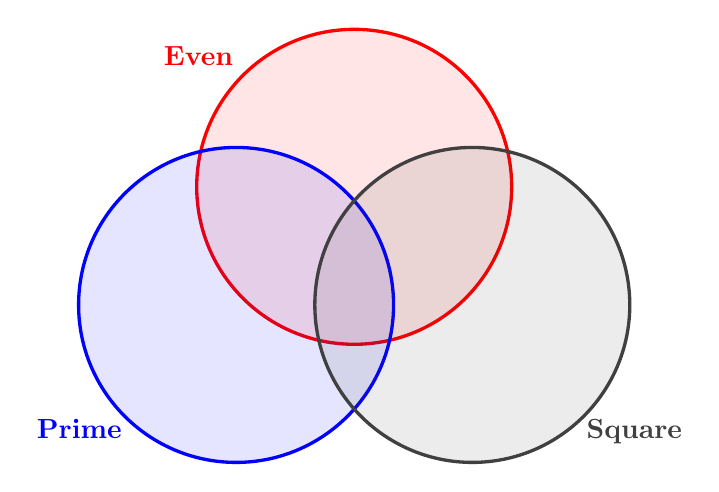
\begin{tikzpicture}
      \draw[very thick,draw=red, fill=red, fill opacity=0.1] (0,0) circle [radius=2cm];
      \draw[very thick,draw=blue,fill=blue,fill opacity=0.1] (-1.5,-1.5) circle [radius=2cm];
      \draw[very thick,draw=black!75,fill=black!75,fill opacity=0.1] (1.5,-1.5) circle [radius=2cm];
      \node[color=red, anchor=south east] at (135:2cm) {\textbf{Even}};
      \node[color=blue, anchor=north east] at (225:4cm) {\textbf{Prime}};
      \node[color=black!75, anchor=north west] at (315:4cm) {\textbf{Square}};
    \end{tikzpicture}
  \end{figure*}
\item In your groups, think of three categories of students at City College that don’t overlap.  Draw them on your paper and label the sets.  Then write your names in the appropriate set. (ex.  Taking 1 class, taking 2 classes, taking 3 or more classes)

  \vfill
\item Think of three categories of students at City College that may overlap. (ex.  Female, taking math this semester, takes trolley to school). Draw the sets and insert your groupmates’ names.

  \vfill

  \clearpage
\item Explain your interpretation of the figure below:

  \begin{figure*}[h!]
    \centering
    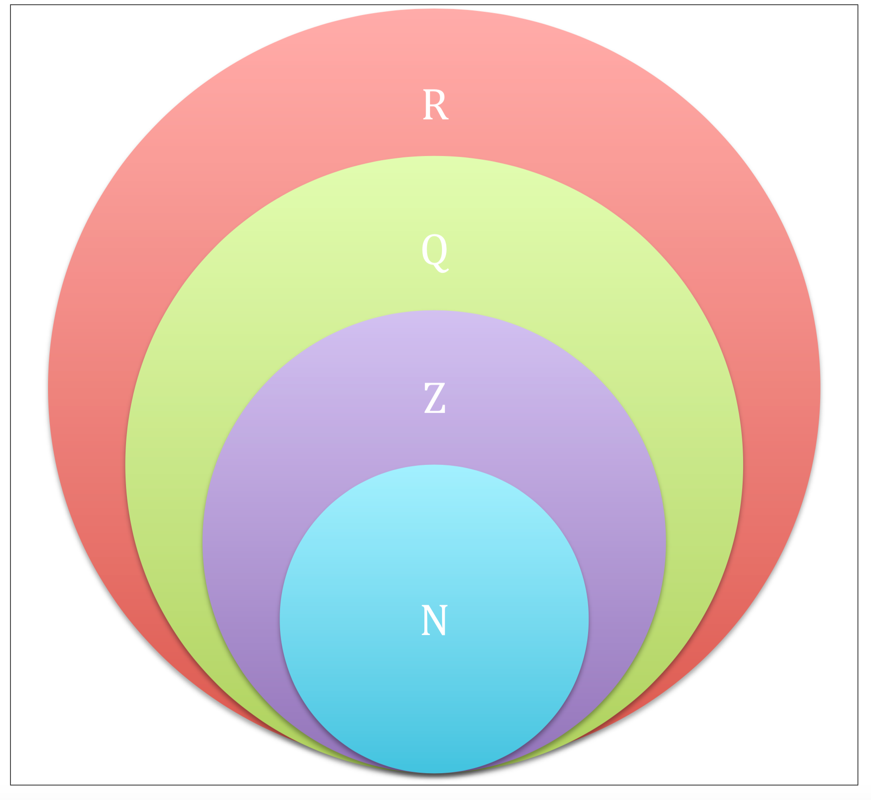
\includegraphics[width=0.4\textwidth]{numbers.png}
  \end{figure*}

  Place the following numbers in the appropriate location above:
  \[
    \left\{5.3,\frac12,-8,0,14,\pi\right\}
  \]
\item Determine of the following statements are true or false. If they are false, correct the statement using proper notation. Box your answer.
  \begin{itemize}
    \ispace{0.25in}
  \item \(\{1,2\} \subseteq \Zn\)
  \item \(\frac12 \in \Zn\)
  \item \(\Rn \subseteq \Zn\)
  \item \(\frac05 \in \Qn\)
  \item \(\frac60 \in \Qn\)
  \item \(\frac70 \in \Rn\)
  \item \(\frac12 \in \Qn\)
  \item \(\Zn \subseteq \Qn\)
  \end{itemize}
  \vspace{0.25in}
\item What is the difference between the symbols \(\in\) and \(\subseteq\)?
\end{enumerate}

\clearpage

\section*{Homework exercises}
Decide whether the following statements are true or false.

\Large

\begin{enumerate}
  \setlength{\itemsep}{\fill}
\item \(3\in\set{7,4,-10,17,13,3,9,67}\)
\item \(4\in\set{14,44,43,24}\)
\item \(\frac13\in \Zn\)
\item \(-5\in \Nn\)
\item \(-\frac{271}{113}\in \Qn\)
\item \(-37\in\Zn\)
\item \(5\in\Rn\)
\item \(\set{2,4,7}\subseteq \set{-3,2,5,4,7}\)
\item \(\set{2,3,5}\subseteq \set{2,5}\)
\item \(\set{2,5,9} \subseteq \set{2,4,9}\)
\item \(\set{-15,\frac34,\pi}\subseteq \Rn\)
\item \(\set{-15,\frac34,\pi}\subseteq \Qn\)
\item \(\set{-2,3,0}\subseteq \Nn\)
\item \(\set{-2,3,0} \subseteq \Zn\)
\item \(\set{\sqrt{2},271}\subseteq \Rn\)
\item \(\set{\sqrt{2},271}\subseteq \Qn\)
  \vfill
\end{enumerate}

\end{document}
%%% Local Variables:
%%% mode: latex
%%% TeX-master: t
%%% End:

